\chapter{Simulating Parallel Imaging}
\label{chapterlabel4}

Following on from the last chapter, which discussed existing simulation strategies, this chapter will focus on how parallel imaging was implemented in POSSUM, from generating sensitivity profiles for the coils, to SENSE image reconstruction. This chapter will also describe SENSE in more detail.

%%%%%%%%%%%%%%%%%%%%%%%%%%
\section{Introduction}
The MRI simulation software used in this thesis is called \textit{Physics Oriented Simulated Scanner Utility for MRI}, or \textit{POSSUM}, and it is part of FSL (FMRIB's Software Library) \footnote{Created by the Analysis Group, FMRIB, Oxford, UK  \url{http://fsl.fmrib.ox.ac.uk/fsl/fslwiki/FSL}}. It is a Bloch equation based simulator which consists of several modules that work together in order to produce a realistic MRI image. This process can be seen in Figure~\ref{fig:possumsim}.  

As stated before, the main goal of this simulator is to produce realistic MRI images given a set of input objects. For that reason, in the remaining of this section the focus will be on the inputs to the simulator that were used in our simulations and will describe them in more depth: 

\begin{figure}[H]
    \centering
    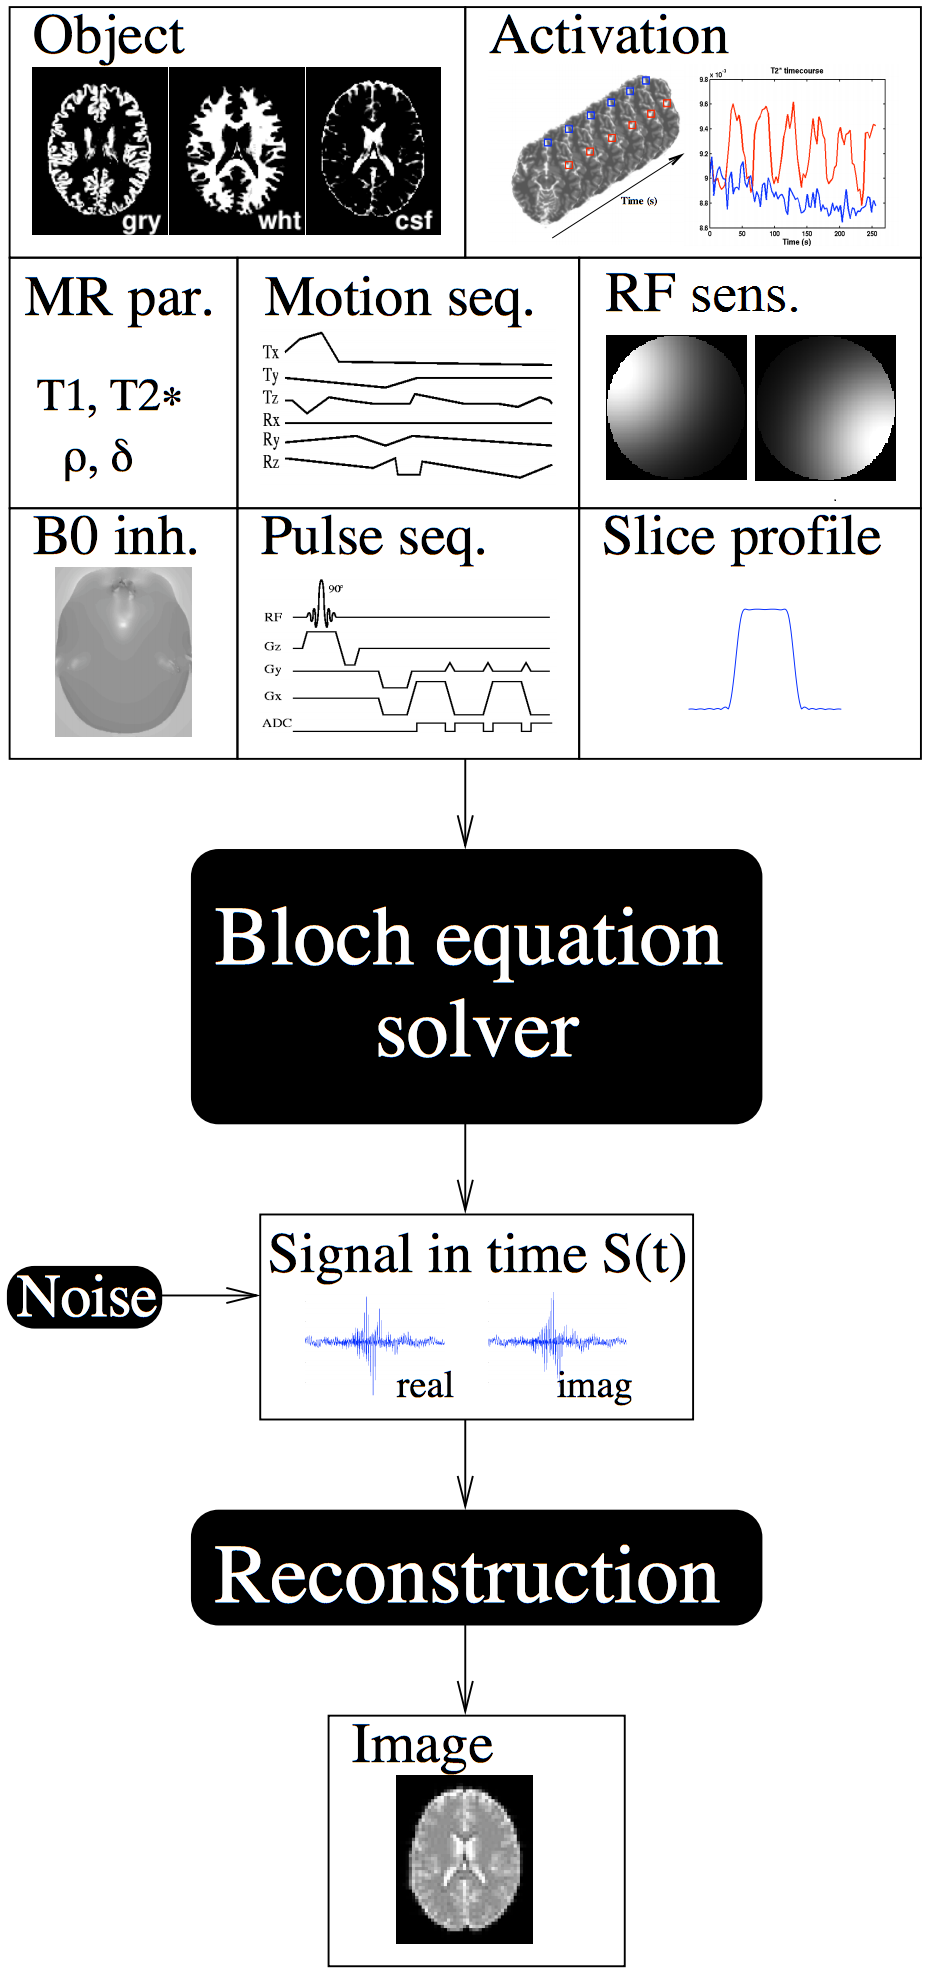
\includegraphics[width=.7\textwidth,keepaspectratio]{possumsim2}
    \caption{POSSUM simulation process in which the Bloch equation solver module receives as input: the object, motion sequence, pulse sequence, $B_0$ inhomogeneities, MR parameters, RF coil sensitivity profiles, slice profile, etc., it produces a signal, adds noise to it and then reconstructs the signal into an image using Fast Fourier Transform (FFT). Figure courtesy of: \cite{Drobnjak07}. Figure was modified to incorporate \textbf{RF coil sensitivity profiles}.}
    \label{fig:possumsim}
\end{figure}

\textit{The object} that POSSUM works with is a four-dimensional anatomical voxel model consisting of different tissue types. For the brain model, 3 tissue types are used: white matter, gray matter, and cerebro-spinal fluid, as seen in Figure~\ref{fig:tissuetemp}. The anatomical models used in POSSUM were produced by the group from McConnell Brain Imaging Centre, Montreal Neurological Institute, McGill University \cite{Kwan1999}, \cite{Cocosco1996}, \cite{Collins1998}. The brain model used in this thesis is made up of 192 x 192 x 192 cuboid voxels of 1mm x 1mm x 1mm in size. Each element contains a value between 0 and 1, representing the proportion of a particular type of tissue in that voxel.

\begin{figure}[H]
    \centering
    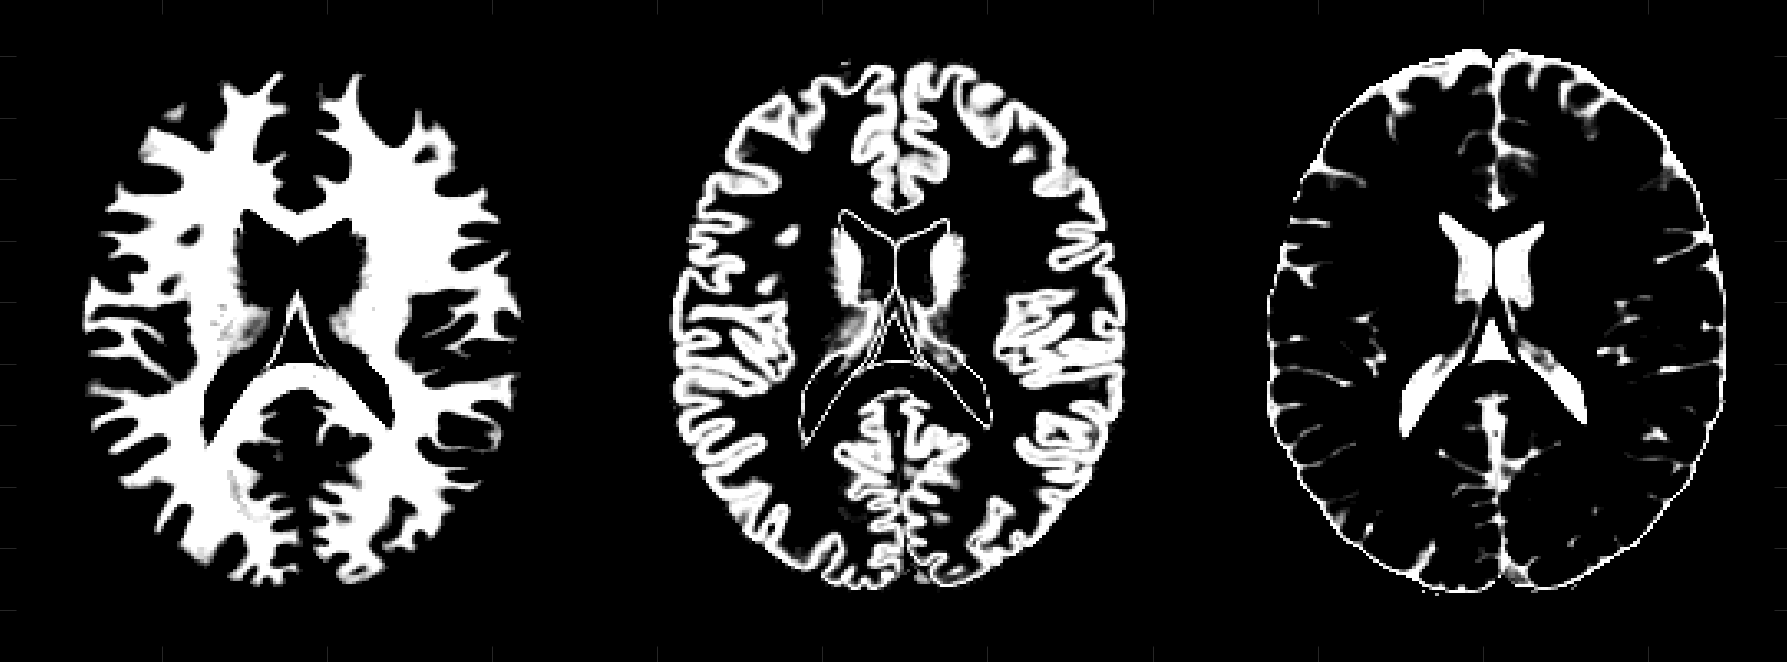
\includegraphics[width=.7\textwidth,keepaspectratio]{tissuetemp}
    \caption{Cross-section tissue templates example showing, from left to right, white matter, gray matter and cerebrospinal fluid}
    \label{fig:tissuetemp}
\end{figure}

\textit{The MR parameters} (relaxation times and spin density $\rho$) for each tissue type in the brain model are offered as input to POSSUM in the form of a matrix. The values for the three tissue types described before were derived by the same group which created the digital brain phantom and can be found in Table~\ref{tab:mrparams}. These values were used throughout all of the simulations from this thesis.

\begin{table}[h!]
\centering
\begin{tabular}{||c c c c ||} 
 \hline
 Tissue Type & $T_1$ (ms) & $T_2^*$ (ms) & $\rho$   \\ [0.5ex] 
 \hline\hline
 Gray Matter & 833 & 83 & 0.86   \\ 
 White Matter  & 500 & 70 & 0.77   \\
 CSF  & 2569 & 329 & 1 \\
 \hline
\end{tabular}
\caption{The MR parameters used in this thesis for different tissue types}
\label{tab:mrparams}
\end{table}

\textit{The pulse sequence} is defined as a series of values in matrix form for the gradients (frequency encoding, phase encoding and slice select), for the RF pulse (angle, frequency bandwidth and frequency centre parameters) and for the signal read-out times. An example of how this table looks like can be seen in Figure~\ref{fig:pulseseqtable}. Also, it is worth mentioning, that the current version of POSSUM simulates two very common pulse sequences, EPI (Echo Planar Imaging) and GE (Gradient Echo), with the possibility to provide a user-defined sequence as well.

\begin{figure}[H]
    \centering
    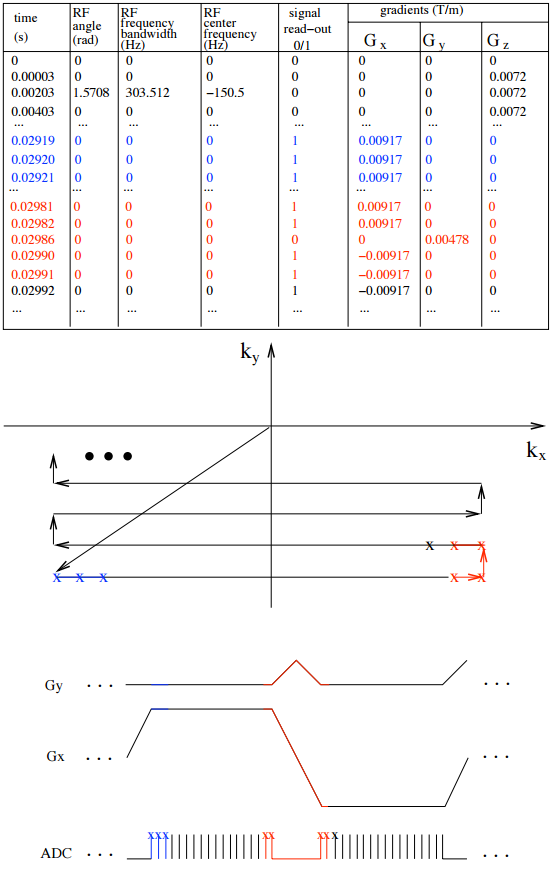
\includegraphics[width=.7\textwidth,keepaspectratio]{pulseseqtable2}
    \caption{The pulse sequence matrix for the POSSUM EPI sequence together with the k-space trajectory. Figure courtesy of \cite{Drobnjak07}}
    \label{fig:pulseseqtable}
\end{figure}

\textit{The motion sequence} can be specified as a file containing values for time (in seconds), for translations ($T_x$, $T_y$ and $T_z$, in meters) and for rotations ($R_x$, $R_y$ and $R_z$, in radians) about the centre of the volume.

\textit{The slice profile} is given in terms of a matrix where the first column specifies the frequency and the second one specifies the amplitude of the RF pulse. The slice profile used in my simulations was derived from a Varian 3T scanner and has a realistic profile which can be viewed in Figure~\ref{fig:sliceprof}. 

\begin{figure}[H]
    \centering
    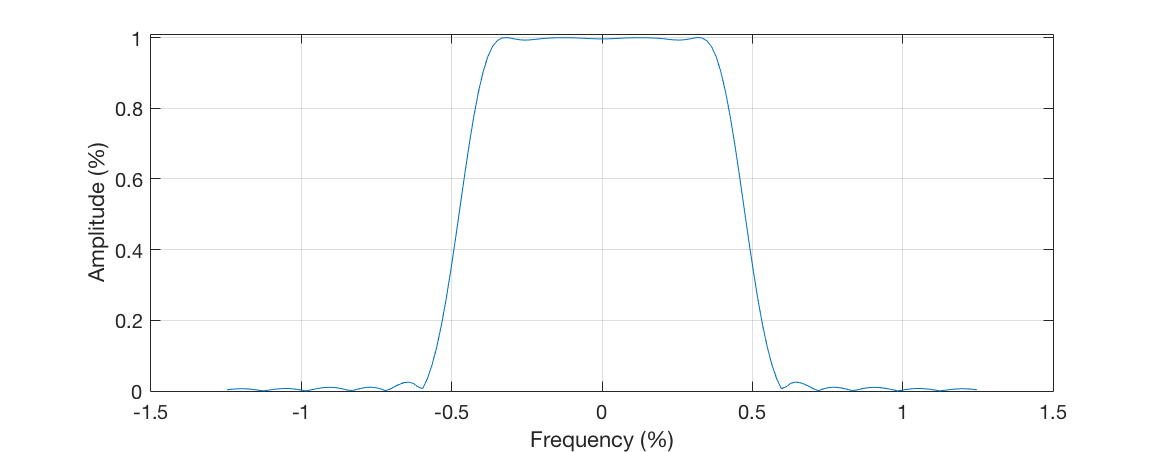
\includegraphics[width=1\textwidth,keepaspectratio]{slcprof}
    \caption{The windowed-sinc RF pulse envelope shape used in POSSUM}
    \label{fig:sliceprof}
\end{figure}

In addition to these input objects, we have created an input object called \textit{coil sensitivity profiles} which will be used for parallel imaging. The next section will cover their implementation and usage in POSSUM.

%%%%%%%%%%%%%%%%%%%%%%%%%%
\section{Coil Sensitivity Profiles}
As has been discussed before, all parallel imaging techniques rely on some knowledge of the multichannel receiver array. Each individual coil from this array has its own sensitivity profile which is dependent on the coil's position with respect to the object being imaged. These maps also show how each individual coil is sensitive to the signal coming from a different spatial location of the desired field of view. As an example, consider an array of 8 coils uniformly distributed in a circle around an object of interest. As shown in Figure~\ref{fig:8coils}, these coils will be sensitive to the signal coming from a limited region of the object.

\begin{figure}[H]
    \centering
    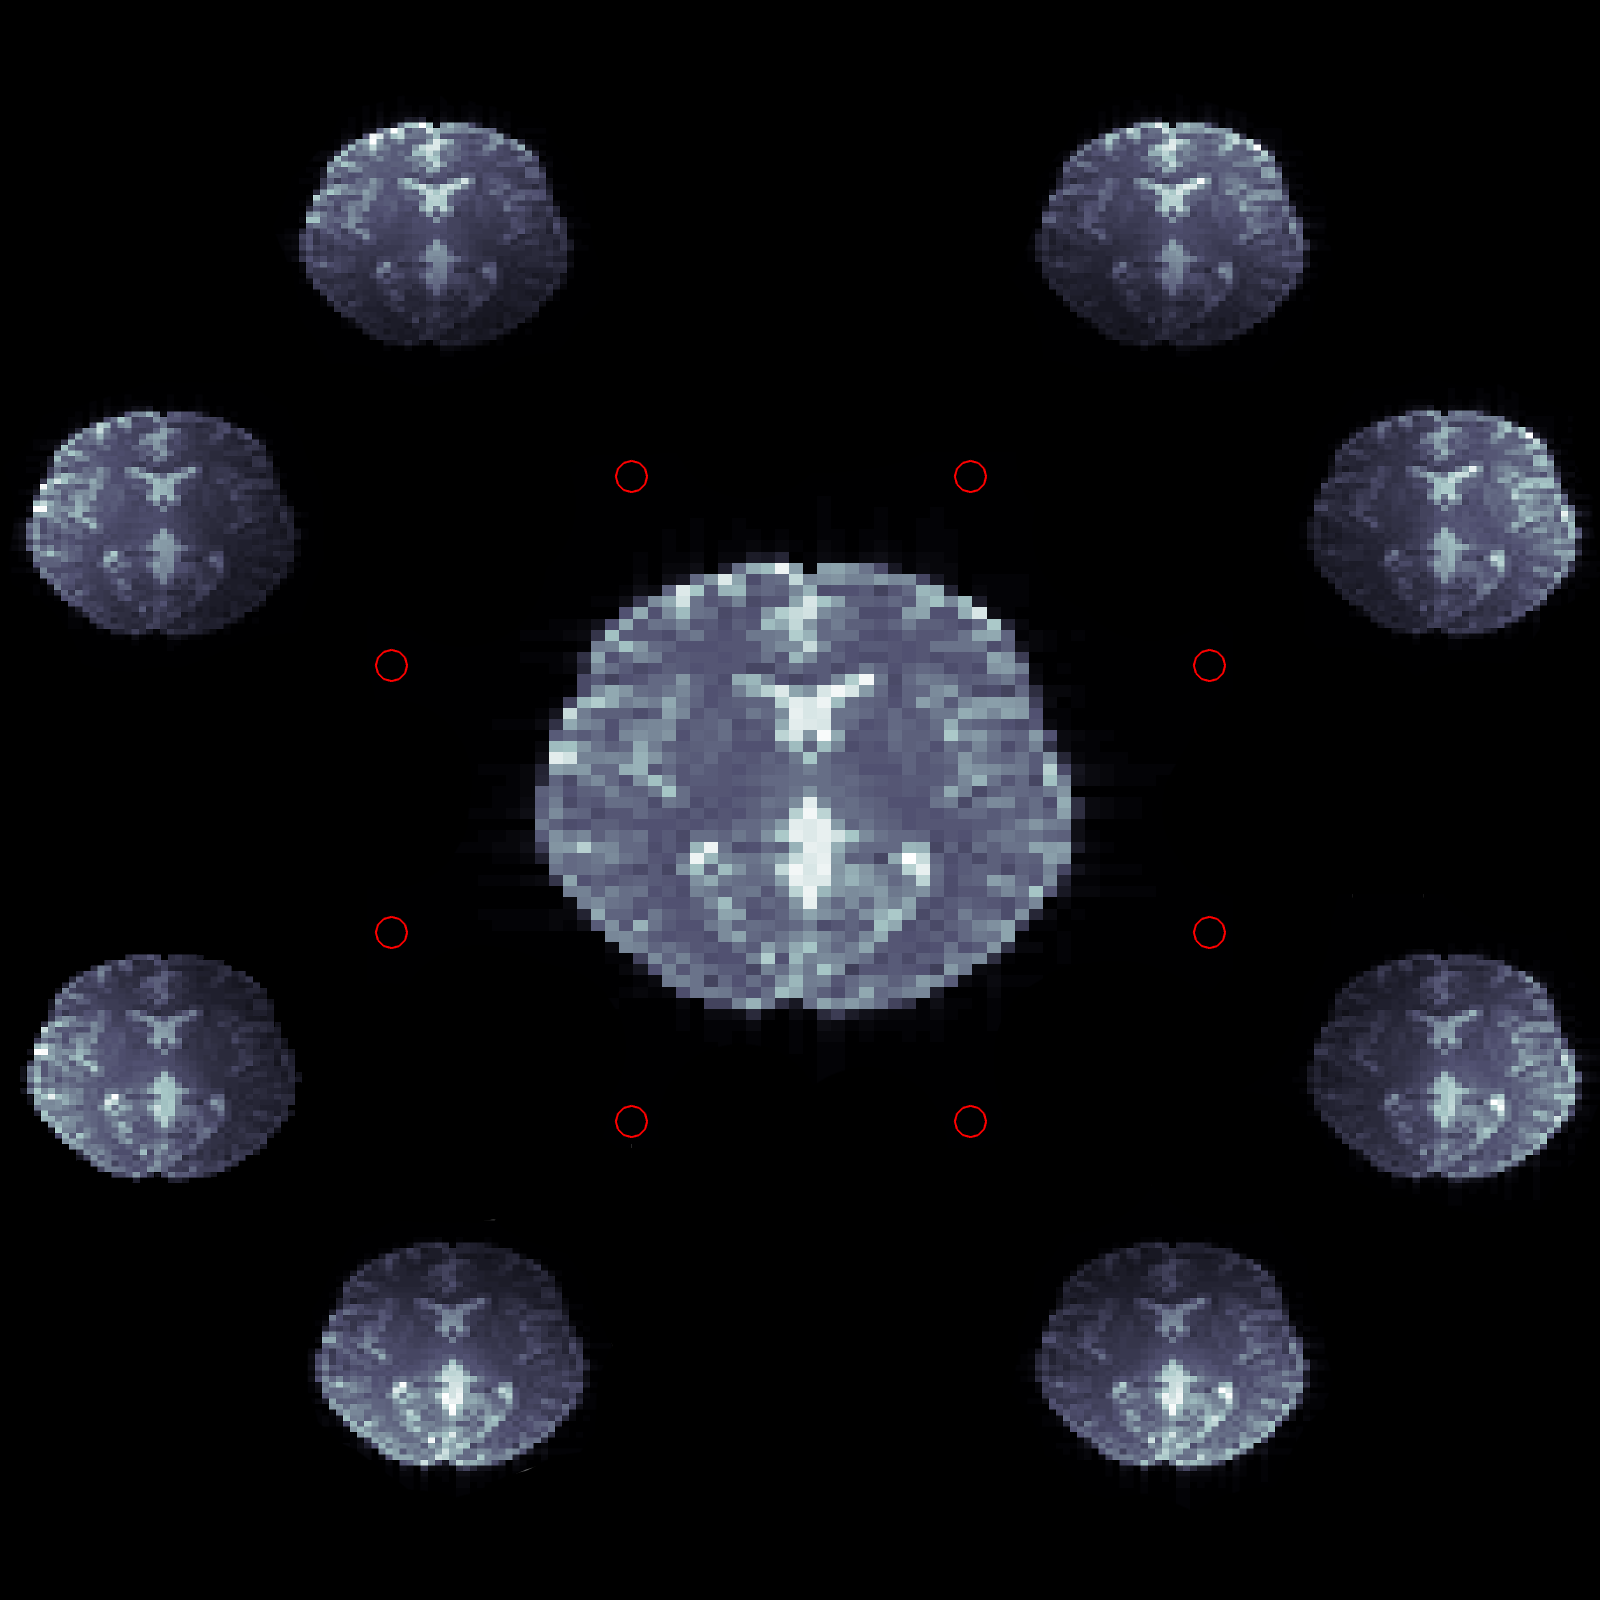
\includegraphics[width=1\textwidth,keepaspectratio]{9brains}
    \caption{An example of a head multichannel receiver array made up of 8 coils. Each red circle is the position of one of the channels}
    \label{fig:8coils}
\end{figure}

In a clinical setting, these coils will be arranged around the object of interest in such a way that each individual coil will cover only part of the FOV and, when put together, they will cover the full FOV. One application that results in increased signal-to-noise ratio \cite{Hayes1991} is to collect the signal from each channel, reconstruct the images and combine them into one final image using a sum-of-squares operation \cite{Roemer1990} or using more sophisticated methods such as those proposed by Walsh et al \cite{Walsh2000}. In addition, great care is taken with how the array is arranged to provide the best possible results, as different body parts have different requirements. For example, a head coil will be arranged in a circular fashion, while a spine array will be linear. Clinically, such arrays can be comprised of 4, 8 and can go up to 32 channels, depending on the application. Each of these coils can have a changing sensitivity in 2 or 3 directions. Since coil sensitivity profiles can provide the extra information missing when parallel imaging is desired, acceleration can occur only in the direction of sensitivity variation. For instance, in case the phased-array coil arrangement is as shown in Figure~\ref{fig:5coils}, parallel imaging will be possible only in the direction of variation between coils, and it will not be possible in the horizontal direction where coil sensitivities do not change \cite{Deshmane2012}. Moreover, in a clinical setting, phased array coils are arranged such that their channels provide maximum variation in the standard phase-encoding directions. 

\begin{figure}[H]
    \centering
    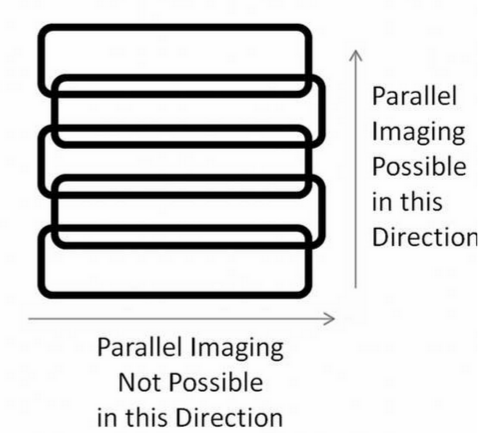
\includegraphics[width=.6\textwidth,keepaspectratio]{5coils}
    \caption{Parallel imaging possible in direction of coil sensitivity variation. Figure courtesy of \cite{Deshmane2012}}
    \label{fig:5coils}
\end{figure}

Turning to an individual coil, it is interesting to investigate more closely how each channel will change the MR image given its intrinsic non-homogeneous sensitivity profile. An example of this can be found in Figure~\ref{fig:1coil} where an object, such as the brain slice found in the left hand side of the figure, is weighted by the sensitivity profile of a given coil (middle image), resulting in the MR image as seen by that channel (right hand side of the figure). Mathematically, this says that each voxel's intensity value from the final image is the result of weighting each voxel's intensity value from the object image by the coil's sensitivity at that location.

\begin{figure}[H]
    \centering
    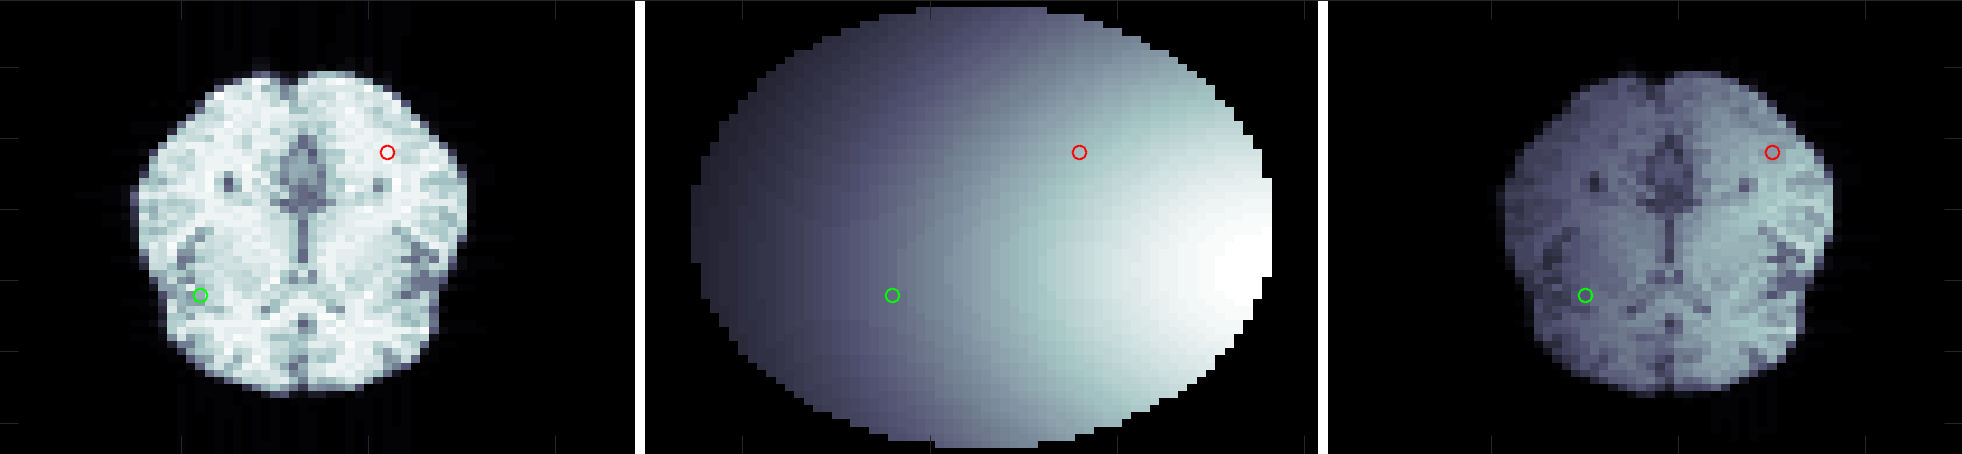
\includegraphics[width=1\textwidth,keepaspectratio]{1coil}
    \caption{From left to right this figure shows: the object, the coil's sensitivity profile and the resulting image as seen by the coil}
    \label{fig:1coil}
\end{figure}

That being said, it is worth investigating how different sensitivity profiles will affect the final reconstruction. Consequently, for this project we have created sensitivity maps that resemble the ones used in parallel imaging techniques. We have opted for a circular geometric placement around the object of interest, with each individual channel being equally apart from its nearest neighbours. Also, we have chosen to spatially vary their sensitivities by modelling a 2D normal distribution which is centered on the channel's position and can have various standard deviations. An example of 2, 4, 6, 8 and 16 channel arrays with sensitivity maps of similar standard deviations is given in Figure~\ref{fig:brainsAndCoilsDistrib}. Moreover, the maps are not spatially varying on the third axis, as the focus for this project was on reconstructing individual slices.

\begin{figure}[H]
    \centering
    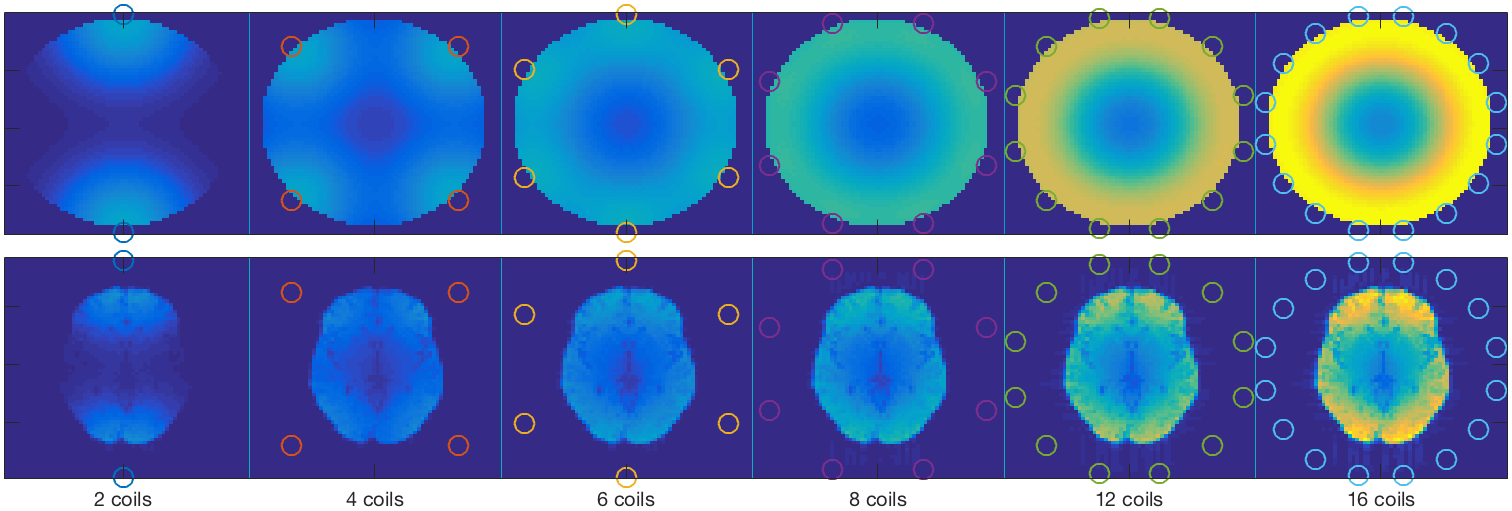
\includegraphics[width=1\textwidth,keepaspectratio]{brainsAndCoilsDistribn2}
    \caption{The 2, 4, 6, 8, 12 and 16 channel arrays used throughout this thesis}
    \label{fig:brainsAndCoilsDistrib}
\end{figure}

As stated before, parallel imaging reconstructions work better when the sensitivity profiles of the channels are spatially varying on the phase-encoding axis, which, in our case, is the y- (vertical) axis of the object. For this reason, as can be seen in Figure~\ref{fig:brainsAndCoilsDistrib}, for the arrays which are made up of 2, 4, 6 and even 8 coils, their geometrical position was chosen such that their spatial variation happens primarily along that axis. For arrays where the number of channels is above 8, that requirement is no longer available as some of the channels will be spatially varying on the x- (horizontal) axis primarily. 

\begin{figure}[H]
    \centering
    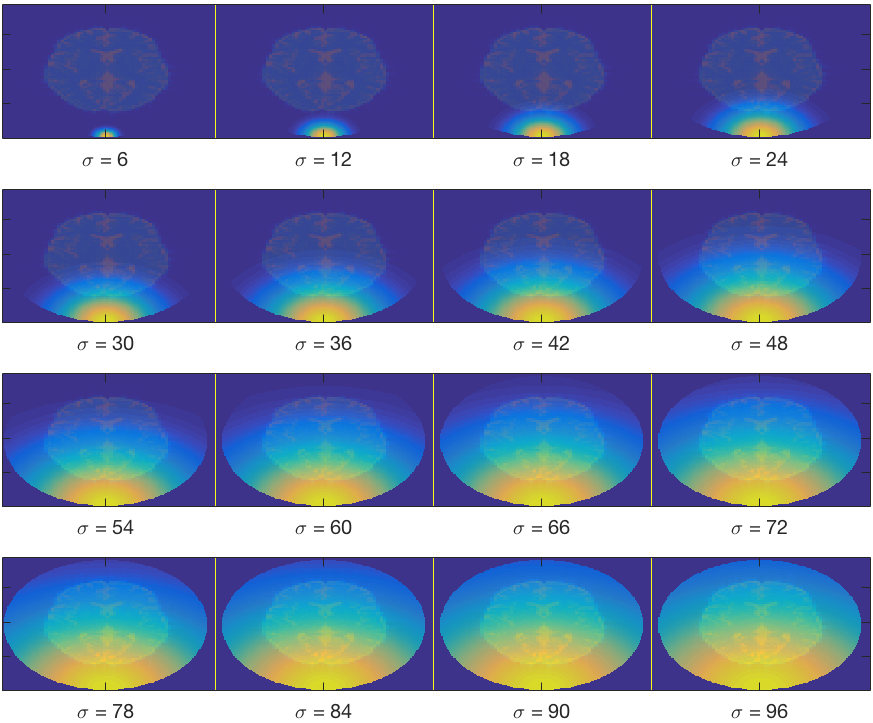
\includegraphics[width=1\textwidth,keepaspectratio]{1coildifsigmas}
    \caption{The sensitivity profiles of an individual channel for increasing standard deviations of the normal distribution used to model their spatial variation}
    \label{fig:1coildifsigmas}
\end{figure}

Another important condition for allowing reasonable reconstructions is to have little overlap between the different coils in order for each individual channel to provide the spatial information needed for a particular area. For this reason, we have chosen to generate sensitivity maps with different coverage sizes to test this theory at the reconstruction step. Figure~\ref{fig:1coildifsigmas} shows the sensitivity profiles of one channel from the 2-coil phased array for different standard deviations of the normal distributions.
%of the individual channels' signal intensity. 
As stated before, the Gaussian distributions model how the signal intensity varies across the object for each individual channel. As expected, a smaller standard deviation will translate into less field-of-view coverage and little overlap, while a higher standard deviation will cover the entire field-of-view and have more overlapping areas between coils. This phenomenon can be visualised in Figure~\ref{fig:2coilsdifsigmas} where the 2-coil array arrangement is presented.

\begin{figure}[H]
    \centering
    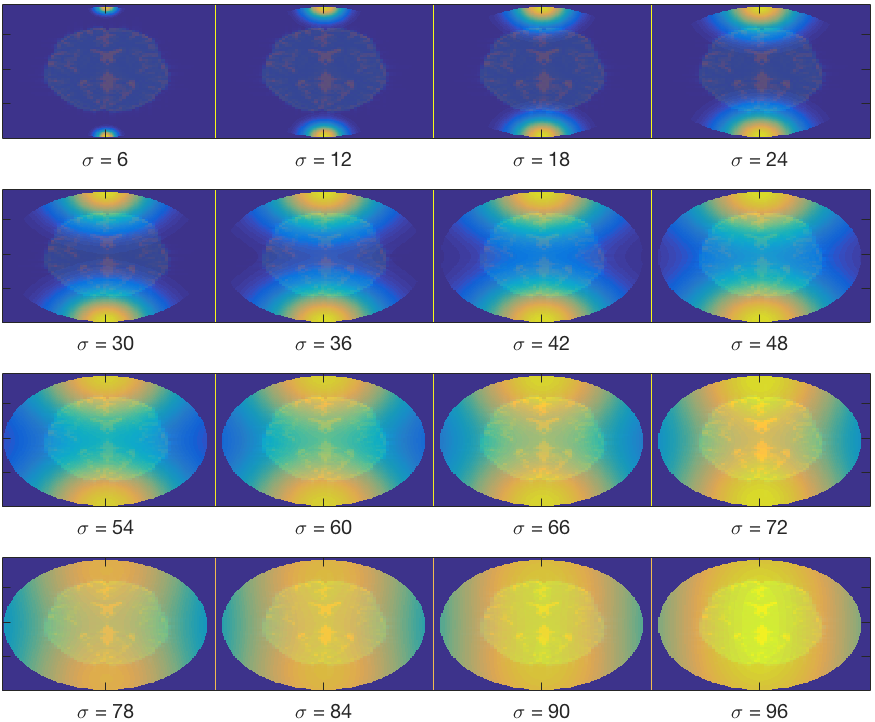
\includegraphics[width=1\textwidth,keepaspectratio]{2coilsdifsigmas}
    \caption{The sensitivity profiles of the 2 channel array}
    \label{fig:2coilsdifsigmas}
\end{figure}

%%%%%%%%%%%%%%%%%%%%%%%%%%
\section{Simulating parallel imaging in POSSUM}
Following on from the previous section which considered the method used to generate coil sensitivity profiles, this section is concerned with how these have been used in the MR simulation pipeline. As mentioned before, the implementation was done within POSSUM, the FMRIB \footnote{Oxford Centre for Functional MRI of the Brain} software tool for simulating realistic MRI and fMRI images. This section will cover in greater detail the MR simulation process when coil sensitivity profiles are present.

To begin with, we will discuss how the signal model is implemented in POSSUM. The simulation process is based on solving the Bloch equations for each individual object voxel at each time point. The overall signal is then calculated as a sum over all magnetization vectors given by the following formula:

\begin{equation} \label{eq:41}
    S(t) = \int_{sample} M_{\perp} (\vec{r}, t) d \vec{r}
\end{equation}
which can be approximated with high accuracy with its discrete form:

\begin{equation} \label{eq:42}
    S(t) = \sum_{j \in \Lambda} \sum_{\vec{r}_0 \in \Omega} s_j (\vec{r}_0, t)
\end{equation}
where $\Omega$ is the set of all object voxels and $\Lambda$ is the set of all tissue templates. 

Therefore, the final signal at time $t$ is given by the sum over all signals $s_j (\vec{r}_0, t)$ coming from the $j$th tissue component at position $\vec{r}_0$ in the input object at time $t$. This is a nice property of the simulator as it allows for tracking of the signal through time and it also allows for various realistic scanning conditions to be implemented. Out of many such scenarios, a few examples can be mentioned: $B_0$ inhomogeneities, RF inhomogeneities and also receiver coil sensitivity profiles can be investigated.

That being said, the first step towards simulating parallel imaging in POSSUM was to add an extra component to the signal calculation. In equation \ref{eq:41} a simplification has been made by considering the receiver coil's sensitivity against the magnetization vector generated by each point of the sample to be equal, and was therefore discarded. In reality, the head coils have an intrinsic sensitivity map which we want to simulate and use. Thus, equation \ref{eq:41} becomes:

\begin{equation} \label{eq:43}
    S(t) = \int_{sample} M_{\perp} (\vec{r}, t) B(\vec{r}) d \vec{r}
\end{equation}
which, again, can be approximated with its discrete version:

\begin{equation} \label{eq:44}
    S(t) = \sum_{j \in \Lambda} \sum_{\vec{r}_0 \in \Omega} s_j (\vec{r}_0, t) B(\vec{r}_0)
\end{equation}

As discussed before, the final signal is the sum over all signals coming from every point in the input object. This object, representing a brain, is made up of 192 x 192 x 192 cuboid elements (of 1mm x 1mm x 1mm in size) which contain information about the properties of each tissue type ($T_1$ and $T_2^*$ relaxation times and spin density $\rho$). These values are uniform across each object voxel. 

That being said, the sensitivity maps of each receiver coil were generated to be of the same size as the input object. In our case, each sensitivity profile is a three dimensional object of 192 x 192 x 192 in size and it contains, for each object voxel, a value between 0 and 1. This value represents how sensitive that respective coil is to the signal coming from a certain spatial location within the object.

As far as different phased-array arrangements is concerned, we have chosen to generate each sensitivity map separately. This implies that, for each mixture of channel positions, we are generating the required number of sensitivity maps and we are running POSSUM with each of them separately. This design choice allows for faster simulations as the software can be run on a cluster system and each coil will be treated by a different job, in parallel.

In practical terms this translates into running the newly enhanced \texttt{possumX} (the CLI\footnote{command line interface} for POSSUM) with the \texttt{-p} flag followed by the number of coils desired. When doing so, you should make sure the simulation folder contains the sensitivity profiles generated earlier. By default, when the flag is not present, POSSUM calculates the signal by considering an overall homogeneous sensitivity profile. At the end of a simulation, the simulation directory will contain as many output images as there were coils. That being said, an \textit{n}-coil arrangement will produce a collection of \textit{n} images for a given standard deviation. An example of such a simulation for a 6-coil array and with a standard deviation of the Gaussian distribution which models the sensitivity profile of $\sigma = 72$ can be seen in Figure~\ref{fig:brains1sigma}.

\begin{figure}[H]
    \centering
    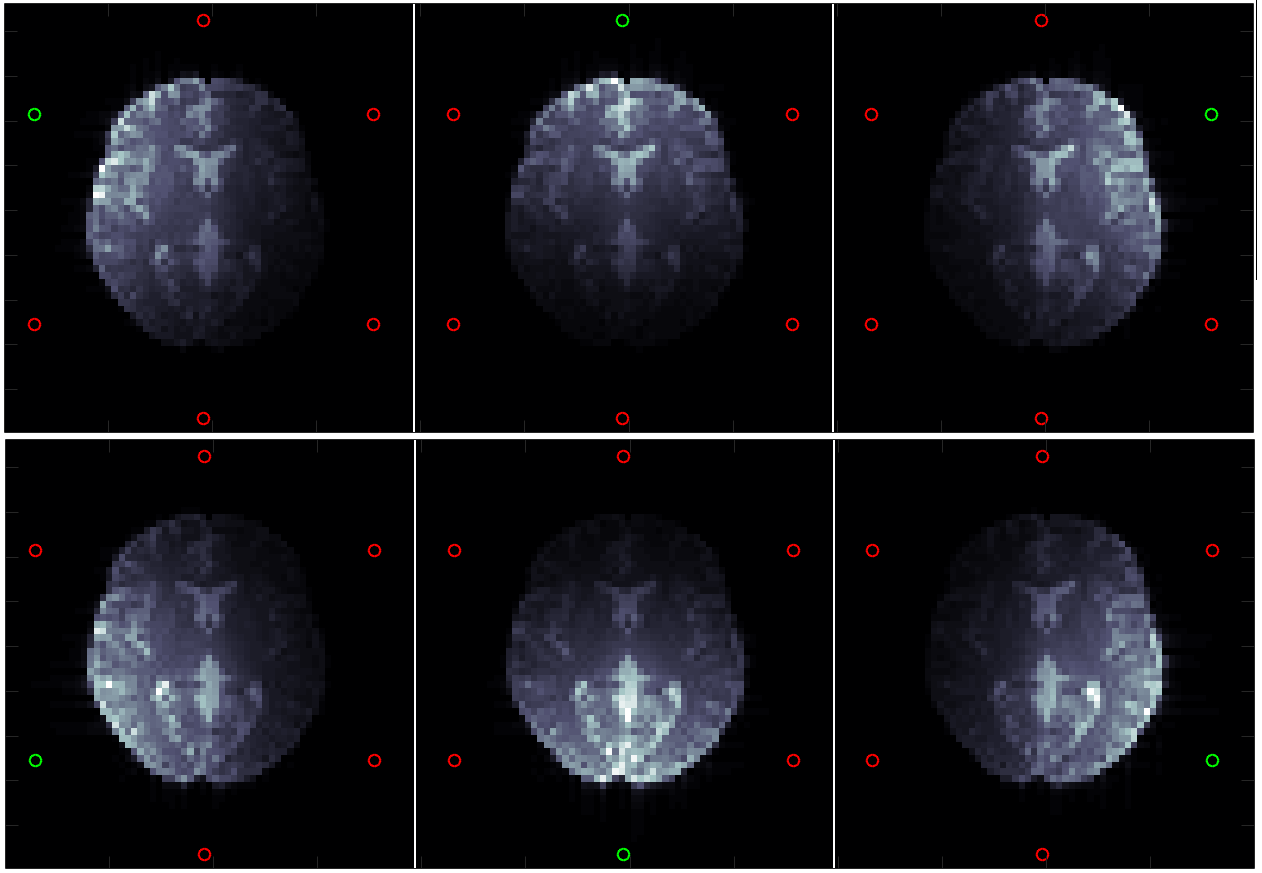
\includegraphics[width=1\textwidth,keepaspectratio]{brains1sigma}
    \caption{A 6-channel phased-array coil simulation for sensitivity maps of $\sigma = 72$}
    \label{fig:brains1sigma}
\end{figure}

%An example of a 4-array coil simulation (positioned North-South-West-East) which was run with the EPI sequence can be seen in Figure~\ref{fig:4arraycoil}.
% 
% \begin{figure}[H]
%     \centering
%     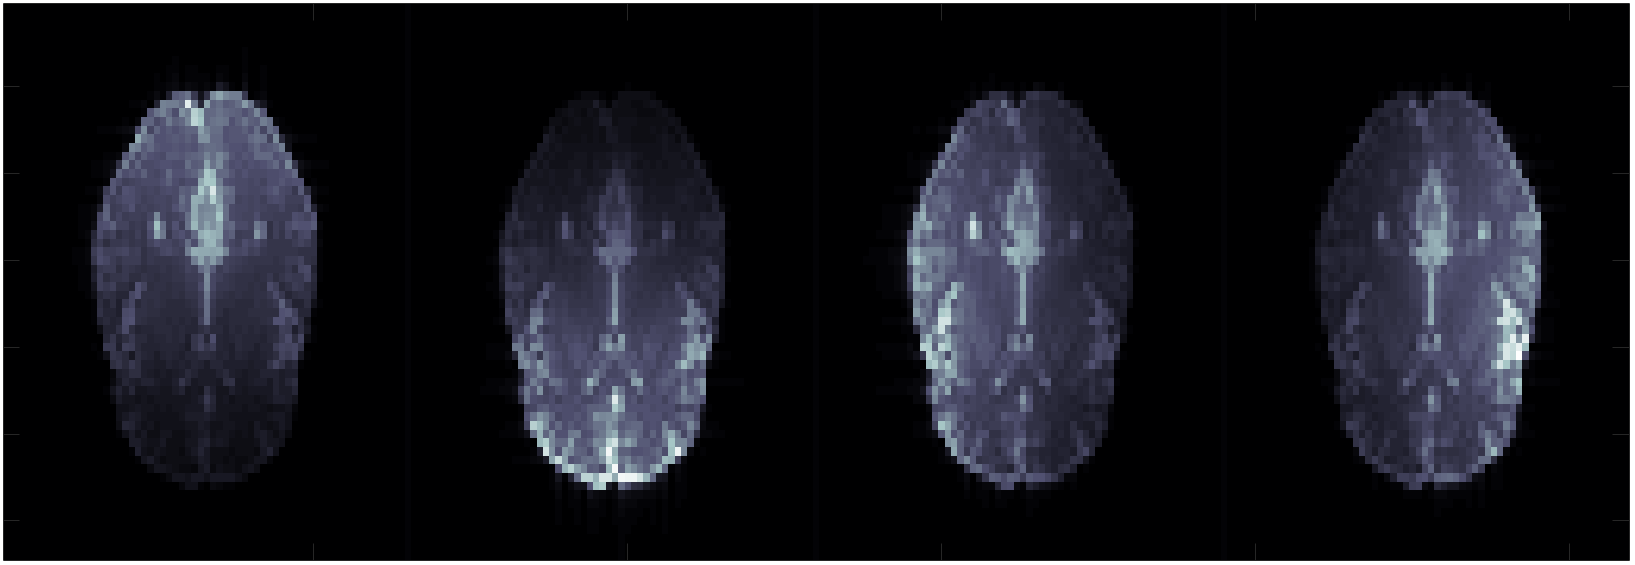
\includegraphics[width=1\textwidth,keepaspectratio]{4arraycoil}
%     \caption{todo caption }
%     \label{fig:4arraycoil}
% \end{figure}

%%%%%%%%%%%%%%%%%%%%%%%%%%
\section{Simulating aliased images in POSSUM}
\label{ch4sectionaliased}
Parallel imaging techniques have been developed in order to accelerate scanning time. As stated before, in order for this to happen, phase-encoding steps can be skipped. The missing information can be recovered by means of coil sensitivity profiles. We have seen in the previous sections how these were generated and then used to reconstruct the final MR image. In this section the focus will be on simulating an undersampled k-space by means of skipping phase-encoding steps.

When an MRI acquisition is performed, each of the scanner's hardware parts, such as the gradients and RF coils, are being controlled by a set of commands sent from the main console. The recipe for how and when to activate different magnetic fields within the scanner is called a pulse sequence. The simulation software has a similar approach as the real scanner in terms of controlling the RF fields, the gradient fields and the receiver electronics. 

To put it more simply, POSSUM defines the pulse sequence as a set of values at discrete time points for the gradient fields and the RF fields. On top of these, the matrix also contains values of $0$s or $1$s for signal read-out ($1$ for when signal should be read and $0$ otherwise). The pulse sequence used by POSSUM is therefore in matrix form which means that user-defined sequences are allowed as long as they preserve the same writing standard. An example was shown in Figure~\ref{fig:pulseseqtable}.

One of the pulse sequences defined by POSSUM is EPI (Echo Planar Imaging) as this software tool was initially designed for fMRI simulations. EPI is a fast imaging technique that allows entire slices to be acquired in one single shot. This means that the entire k-space matrix can be acquired after one RF pulse (for GE-EPI). A diagram of a standard GE-EPI pulse sequence in shown in Figure~\ref{fig:episequence} together with the corresponding k-space acquisition. 

\begin{figure}[H]
    \centering
    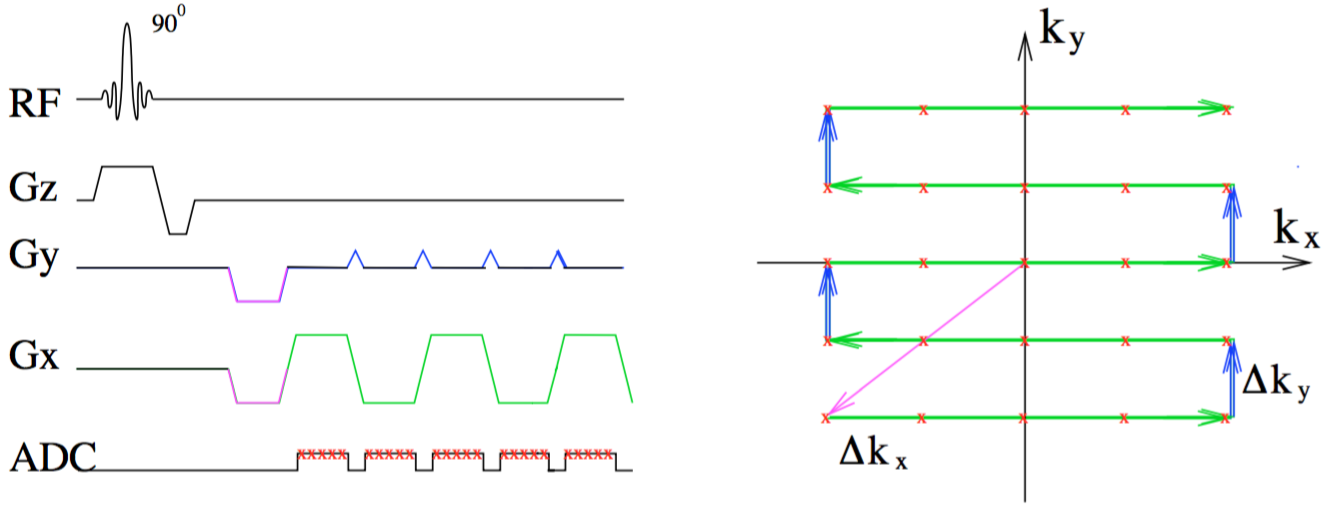
\includegraphics[width=1\textwidth,keepaspectratio]{episequence}
    \caption{Standard echo planar imaging (EPI) sequence together with the corresponding k-space sampling. Figure courtesy of \cite{Drobnjak07}}
    \label{fig:episequence}
\end{figure}

In order to accelerate the image acquisition process, two steps need to be done. First, the phase encoding gradients need to be increased by the same amount as the parallel imaging acceleration factor R. For example, to halve the acquisition time ($R = 2$), the phase encoding gradients, or "blips", need to become twice as strong as in a normal acquisition. This will translate into $\Delta k_y' = 2 \Delta k_y$ which is the same as skipping every other k-space line. Second, the number of k-space lines acquired needs to be decreased by the same factor R. This means that for a standard 128 x 128 k-space matrix, when using $R = 2$, the final k-space size will be reduced to 64 x 128, halving the amount of phase-encoding lines.

As we have discussed before in Chapter~\ref{chapterlabel2}, the 
k-space sampling interval in the phase-encoding direction is inversely proportional to the field-of-view: $\Delta k_y = \frac{1}{FOV_y}$ (eq. \ref{eq:270}). Also, the image spatial resolution is inversely proportional to the highest spatial frequency sampled in k-space. In mathematical terms, this translates into $\Delta y = \frac{1}{N_y \Delta k_y} = \frac{1}{2 k_{y,max}}$ (eq. \ref{eq:273}). This means that for an acceleration factor $R = 2$, the sampling interval will increase twofold leading to: $\Delta k_y' = 2 \Delta k_y = \frac{2}{FOV_y} = \frac{1}{\frac{FOV_y}{2}} = \frac{1}{FOV_y'}$. Therefore, the new field of view is half of the original one: $FOV_y' = \frac{FOV_y}{2}$. This leads to aliasing in the final images as the \textit{Nyquist-Shannon} condition is not met anymore.

This phenomenon was simulated in POSSUM. The results were as expected and the final reconstructions showed aliased images. An example of a simulation ran with an acceleration factor $R = 2$, meaning a halved field-of-view, can be found in Figure \ref{fig:figaliased}. The 6-channel array used was presented in Figure~\ref{fig:brains1sigma}.

\begin{figure}[H]
    \centering
    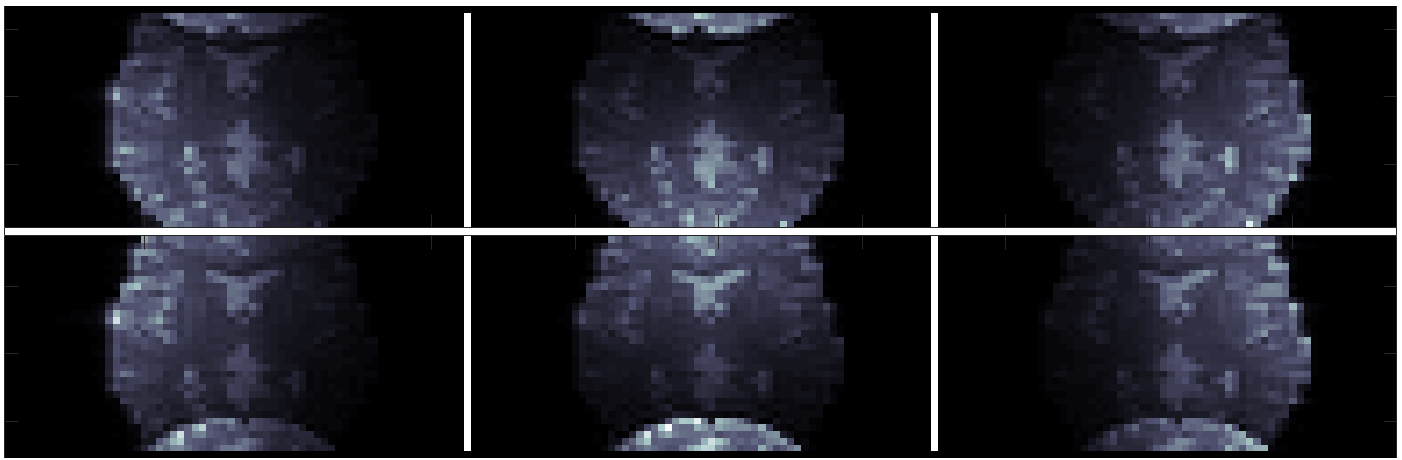
\includegraphics[width=1\textwidth,keepaspectratio]{figaliased}
    \caption{POSSUM simulating aliased images with a 6-coil array and with an acceleration factor $R = 2$}
    \label{fig:figaliased}
\end{figure}

For all our simulations that will be presented in the next chapter, we have used the (parallel imaging capable) Echo Planar Imaging pulse sequence. This is one of the most common MRI pulse sequences for single-shot k-space acquisitions, as it can acquire up to 128 phase-encoding steps in 20-100ms. Although it provides excellent temporal resolution and it is the most popular sequence for fMRI studies, the image quality can be poor \cite{Farzaneh1990}. This is due to various problems associated with this sequence such as signal dropout at the interfaces between different tissue types where magnetic susceptibility differences appear. It was therefore proposed by Griswold et al \cite{Griswold1999} and by Bammer et al \cite{Bammer2001} that the use of parallel imaging techniques can reduce image artifacts to a level that was only accomplished by interleaved EPI acquisitions \cite{Schmiedeskamp2010}. Although the investigation of whether this holds true with simulation is not the scope of this project, it could become future work.

%%%%%%%%%%%%%%%%%%%%%%%%%%
\section{SENSE reconstruction}
\label{ch4sectionsense}
So far we have seen how coil sensitivity maps were generated for various phased-array channel arrangements and how they can be used in POSSUM to simulate signal acquisition with coils that have a non-homogeneous spatial sensitivity. We have also discussed the simulation of aliased images in our MRI software tool. These two together are part of the parallel imaging pipeline being developed in POSSUM. This next section is concerned with the reconstruction algorithm that uses the folded images and the coil sensitivity profiles in order to retrieve the original image.

Pruessmann et al showed in 1999 that for 2D Fourier imaging with k-space coefficients being sampled in a Cartesian fashion, scan time can be reduced by increasing the relative distance between adjacent sampling positions \cite{Pruessmann1999}. This will invariably lead to a reduction of the FOV, causing folding in the final images. However, this is where parallel imaging reconstruction algorithms come into place. As we have discussed before, there are a couple of ways to recover full FOV images from aliased ones. One of these algorithms which does reconstruction in the image domain is SENSE and it is the topic of our discussion in this section.

The main idea behind SENSE (sensitivity encoding) is to use the sensitivity maps of the individual receiver channels in order to 'unfold' the aliased images. It therefore relies on two separate inputs: the set of images reconstructed for each of the individual coils from the multi-coil array and the collection of sensitivity profiles of these channels. Having these two, reconstruction works as long as there are more channels than folded intensities \cite{Pruessmann1999}. 

To better understand this phenomenon, let us follow an example. In Figure~\ref{fig:senserecbrains} we see on the left-hand side of the image the object of interest: a brain. Next, the middle column shows how each individual channel sees the object: every intensity value for each location in the image is weighted by the coil's sensitivity at those coordinates. Finally, in the right hand side column, we can see the reconstructed (aliased) images for each channel. In our example, acquisition was performed with an acceleration factor $R = 2$, which means that the final field-of-view will be halved. For qualitative purposes, the images shown are full FOV, for the purpose of seeing exactly where parts of our initial object are juxtaposing.

Figure~\ref{fig:senserecbrains} also shows that the two locations $A$ and $B$ are 'folded' in the final images, both intensities contributing to the final value found in the aliased images. Therefore, as long as the two locations experience different sensitivity weightings by each of the channels in the phased-array coil, a good reconstruction can be performed.

\begin{figure}[H]
    \centering
    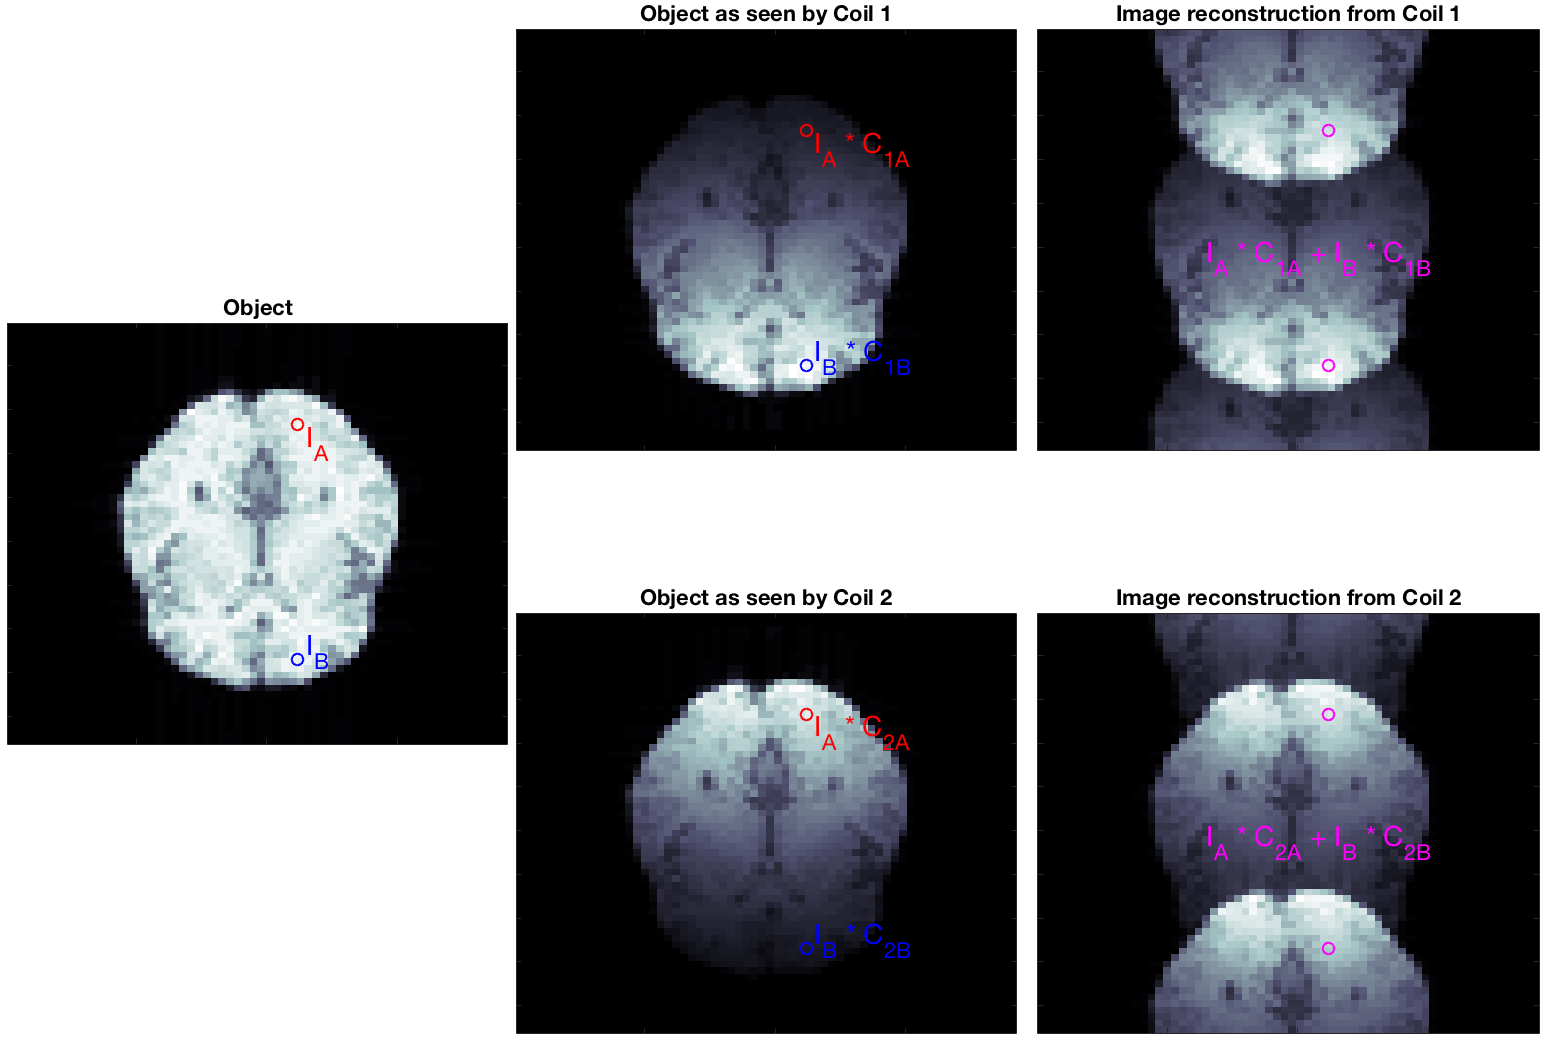
\includegraphics[width=1\textwidth,keepaspectratio]{senserecbrains}
    \caption{Aliased images from two coils. The signal value at folded locations shown in magenta is the sum between the object values at the two locations, A and B, for each coil.}
    \label{fig:senserecbrains}
\end{figure}

Now, in order to express this concept mathematically, a few other aspects need to be discussed. First, we take into account the fact that the acceleration factor $R$ contributes to a reduction of the FOV from $L$ to $L/R$, where $L$ is the length of our full field-of-view. Second, the total number of replicates (overlapping signals) at each voxel location is $N_A = 2 N(AR/L) + 1$, where $N(u) = -[(1-u)/2]$ is defined to be the \textit{largest integer less than or equal to} operation and $A$ is the length of the FOV which encompasses the object of interest. Third, we define the number of channels in the coil array as $N_c$ and the sensitivity profiles for each of them as $C_j$, for $j \in [0, N_c-1]$. Finally, for each location $y$ in the image, we can write the signal intensity $I(y)$ at that location as a sum of the weighted intensity values coming from each of the aliased locations. 

\begin{equation} \label{eq:45}
    I_j(y)  = \sum_{n=0}^{N_A-1} C_j(y+nL/R) M(y+nL/R)
\end{equation}
where $M$ holds the real intensity values from the object of interest for each location $y$.

Now, if $N_c \geq N_A$, the system of equations can be solved and $M(y+nL/R)$ can be retrieved. Writing $I$ as an $N_c$ x $1$ matrix, $C$ as an $N_c$ x $N_A$ matrix and $M$ as an $N_A$ x $1$ matrix, we get:

\begin{equation}
    I = \left[
    \begin{array}{ c }
          I_0(y) \\
          I_1(y) \\
          \cdots \\
           I_{N_c-1}(y)
    \end{array}
    \right],
\end{equation}

\begin{equation}
    C = \left[
    \begin{array}{ c c c }
          C_0(y) & \cdots & C_0(y+(N_A-1)L/R)  \\
          \cdots & \cdots & \cdots \\
          C_{N_c-1}(y) & \cdots & C_{N_c-1}(y+(N_A-1)L/R)
    \end{array}
    \right]
\end{equation}
and
\begin{equation}
    M = \left[
    \begin{array}{ c }
          M(y) \\
          M(y+L/R) \\
          \cdots \\
          M(y+(N_A-1)L/R)
    \end{array}
    \right]
\end{equation}

We can therefore write equation \ref{eq:45} in matrix form as:

\begin{equation}
    I = C M
\end{equation} 

In order to recover the unfolded image, a Moore-Penrose pseudo-inverse is performed:

\begin{equation}
    M = (C^T C) ^{-1} C^T I =  C^\dagger I
\end{equation}

The reconstruction step of the pipeline was implemented in MATLAB following a medical imaging reconstruction tutorial\footnote{\url{https://web.stanford.edu/class/ee369c/restricted/Solutions/assignment_4_solns.pdf}} offered by Stanford. The algorithm requires 3 inputs: the collection of aliased images, the set of coil sensitivity profiles and the acceleration factor R.

Moreover, a function for calculating the coil "g-factor" is implemented as well. The mathematical concepts behind the coil geometry factor have been presented in Section \ref{sect:senserec}. Nevertheless, it is an important notion that needs to be reminded. The coil "g-factor" is a measure of the added noise brought about the combination of multiple coils. It can be calculated with the following equation:

\begin{equation}
    g_y = \sqrt{ [(C^T \Psi^{-1} C )^{-1}]_{yy} (C^T \Psi^{-1} C )_{yy} }
\end{equation}

where $g_y$ is the g-factor at location $y$, $\Psi$ is the noise correlation matrix and $C$ is the sensitivity encoding matrix. This factor also influences the signal-to-noise ratio in the final reconstructed images. The signal drop is given by the next equation:

\begin{equation}
    SNR_{SENSE} = \frac{SNR_{Original}}{g \sqrt{R}}
\end{equation}

where $R$ is the acceleration factor and $SNR_{Original}$ is the signal-to-noise ratio of a similar MRI image taken without parallel imaging.

The simulations which will be presented in the next chapter will use the Stanford tutorial to perform SENSE reconstructions and g-factor maps for a combination of array channels, sensitivity profiles and acceleration factors.













